%%%%%%%%%%%%%%%%%%%%%%%%%%%%%% Preamble
\documentclass[11pt]{article}
\setlength{\parskip}{\baselineskip}%
\setlength{\parindent}{0pt}%
\usepackage{amsmath,amssymb,amsthm,physics,graphicx,titling}
\newcommand{\subtitle}[1]{%
  \posttitle{%
    \par\end{center}
    \begin{center}\large#1\end{center}
    \vskip0.5em}%
}

\usepackage{graphicx}
\begin{document}

%%%%%%%%%%%%%%%%%%%%%%%%%%%%%% Heading
	\title{Ph20 - Assignment 3}
	\author{Yovan Badal}
	\date{12/03/2017}
	\maketitle
	
%%%%%%%%%%%%%%%%%%%%%%%%%%%%%% Body
\section*{Part 1}
1. We implement the explicit Euler method, and use the script to plot $x$ and $v$ as functions of time, for initial conditions $x(0) = 1$, $v(0) = 0$, $h = 0.01$ and $t$ running from 0 to 20.
\begin{figure}[htp]
\centering
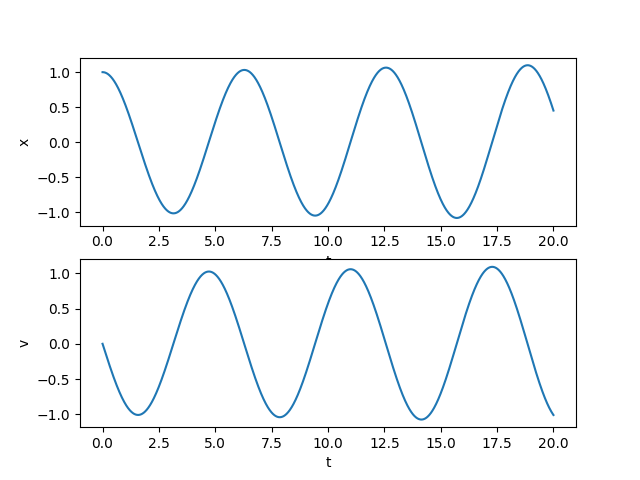
\includegraphics[scale=0.54]{x_and_v_plot_1_0_0.01_20.png}
\caption{Plot of $x$ and $v$ as functions of time for initial conditions $x(0) = 1$, $v(0) = 0$, and stepsize $h = 0.01$.}
\label{explicit}
\end{figure}
\newpage

2. We observe that the analytical solution to the simple harmonic oscillation equation $F = -kx$ for the intial conditions given is $x = \cos(t)$ and $v = -\sin(t)$.

We can compare our numerical solution to the analytic solution by plotting the global errors $x_{analytic}(t_i) - x_i$ and $v_{analytic}(t_i) - v_i$ against time.
\begin{figure}[htp]
\centering
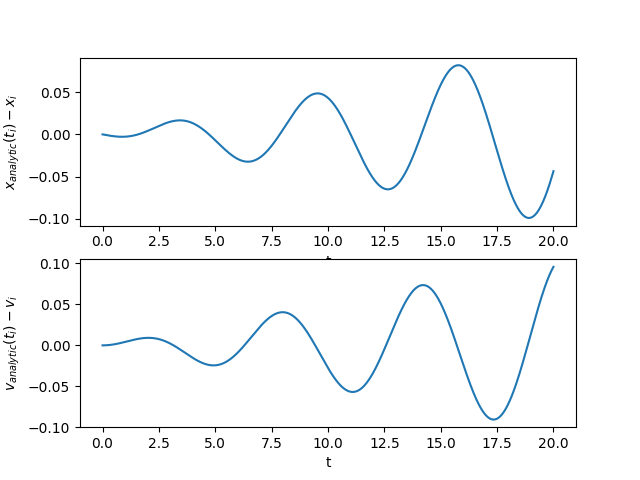
\includegraphics[scale=0.70]{x_err_and_v_err_plot_1_0_0.01_20.png}
\caption{Plot of global errors against time for the explicit Euler method, with stepsize $h=0.01$.}
\label{expliciterror}
\end{figure}
\newpage

3. We now plot the maximum global error in $x$ against $h$, integrating up to the same final time $t = 20$.
\begin{figure}[htp]
\centering
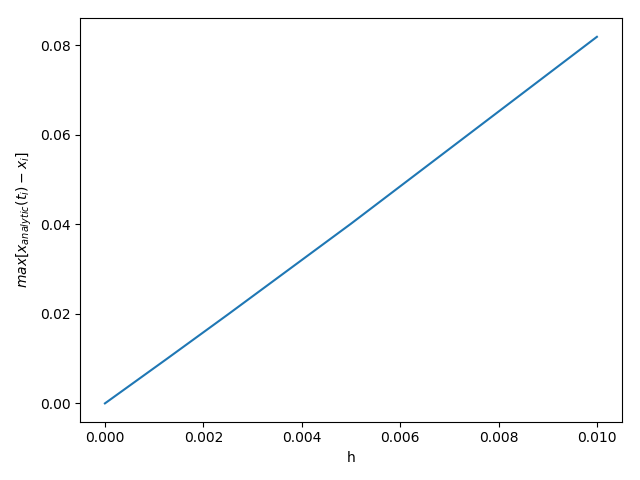
\includegraphics[scale=0.70]{err_behavior_0.01_4_20.png}
\caption{Plot of maximum global error in $x$ against $h$, integrating up to $t=20$ for each $h$.}
\label{expliciterrbehavior}
\end{figure}

The plot indicates that the truncation error is proportional to $h$ for reasonable $h$.


\end{document}